\documentclass[english,man]{apa6}

\usepackage{amssymb,amsmath}
\usepackage{ifxetex,ifluatex}
\usepackage{fixltx2e} % provides \textsubscript
\ifnum 0\ifxetex 1\fi\ifluatex 1\fi=0 % if pdftex
  \usepackage[T1]{fontenc}
  \usepackage[utf8]{inputenc}
\else % if luatex or xelatex
  \ifxetex
    \usepackage{mathspec}
    \usepackage{xltxtra,xunicode}
  \else
    \usepackage{fontspec}
  \fi
  \defaultfontfeatures{Mapping=tex-text,Scale=MatchLowercase}
  \newcommand{\euro}{€}
\fi
% use upquote if available, for straight quotes in verbatim environments
\IfFileExists{upquote.sty}{\usepackage{upquote}}{}
% use microtype if available
\IfFileExists{microtype.sty}{\usepackage{microtype}}{}

% Table formatting
\usepackage{longtable, booktabs}
\usepackage{lscape}
% \usepackage[counterclockwise]{rotating}   % Landscape page setup for large tables
\usepackage{multirow}		% Table styling
\usepackage{tabularx}		% Control Column width
\usepackage[flushleft]{threeparttable}	% Allows for three part tables with a specified notes section
\usepackage{threeparttablex}            % Lets threeparttable work with longtable

% Create new environments so endfloat can handle them
% \newenvironment{ltable}
%   {\begin{landscape}\begin{center}\begin{threeparttable}}
%   {\end{threeparttable}\end{center}\end{landscape}}

\newenvironment{lltable}
  {\begin{landscape}\begin{center}\begin{ThreePartTable}}
  {\end{ThreePartTable}\end{center}\end{landscape}}

  \usepackage{ifthen} % Only add declarations when endfloat package is loaded
  \ifthenelse{\equal{\string man}{\string man}}{%
   \DeclareDelayedFloatFlavor{ThreePartTable}{table} % Make endfloat play with longtable
   % \DeclareDelayedFloatFlavor{ltable}{table} % Make endfloat play with lscape
   \DeclareDelayedFloatFlavor{lltable}{table} % Make endfloat play with lscape & longtable
  }{}%



% The following enables adjusting longtable caption width to table width
% Solution found at http://golatex.de/longtable-mit-caption-so-breit-wie-die-tabelle-t15767.html
\makeatletter
\newcommand\LastLTentrywidth{1em}
\newlength\longtablewidth
\setlength{\longtablewidth}{1in}
\newcommand\getlongtablewidth{%
 \begingroup
  \ifcsname LT@\roman{LT@tables}\endcsname
  \global\longtablewidth=0pt
  \renewcommand\LT@entry[2]{\global\advance\longtablewidth by ##2\relax\gdef\LastLTentrywidth{##2}}%
  \@nameuse{LT@\roman{LT@tables}}%
  \fi
\endgroup}


  \usepackage{graphicx}
  \makeatletter
  \def\maxwidth{\ifdim\Gin@nat@width>\linewidth\linewidth\else\Gin@nat@width\fi}
  \def\maxheight{\ifdim\Gin@nat@height>\textheight\textheight\else\Gin@nat@height\fi}
  \makeatother
  % Scale images if necessary, so that they will not overflow the page
  % margins by default, and it is still possible to overwrite the defaults
  % using explicit options in \includegraphics[width, height, ...]{}
  \setkeys{Gin}{width=\maxwidth,height=\maxheight,keepaspectratio}
\ifxetex
  \usepackage[setpagesize=false, % page size defined by xetex
              unicode=false, % unicode breaks when used with xetex
              xetex]{hyperref}
\else
  \usepackage[unicode=true]{hyperref}
\fi
\hypersetup{breaklinks=true,
            pdfauthor={},
            pdftitle={The N400's 3 As: Association, Automaticity, Attenuation (and Some Semantics Too)},
            colorlinks=true,
            citecolor=blue,
            urlcolor=blue,
            linkcolor=black,
            pdfborder={0 0 0}}
\urlstyle{same}  % don't use monospace font for urls

\setlength{\parindent}{0pt}
%\setlength{\parskip}{0pt plus 0pt minus 0pt}

\setlength{\emergencystretch}{3em}  % prevent overfull lines

\ifxetex
  \usepackage{polyglossia}
  \setmainlanguage{}
\else
  \usepackage[english]{babel}
\fi

% Manuscript styling
\captionsetup{font=singlespacing,justification=justified}
\usepackage{csquotes}
\usepackage{upgreek}

 % Line numbering
  \usepackage{lineno}
  \linenumbers


\usepackage{tikz} % Variable definition to generate author note

% fix for \tightlist problem in pandoc 1.14
\providecommand{\tightlist}{%
  \setlength{\itemsep}{0pt}\setlength{\parskip}{0pt}}

% Essential manuscript parts
  \title{The N400's 3 As: Association, Automaticity, Attenuation (and Some
Semantics Too)}

  \shorttitle{N400 Association Attenuation}


  \author{Erin M. Buchanan\textsuperscript{1}, John E. Scofield\textsuperscript{2}, \& Nathan Nunley\textsuperscript{3}}

  % \def\affdep{{"", "", ""}}%
  % \def\affcity{{"", "", ""}}%

  \affiliation{
    \vspace{0.5cm}
          \textsuperscript{1} Missouri State University\\
          \textsuperscript{2} University of Missouri\\
          \textsuperscript{3} University of Mississippi  }

  \authornote{
    Erin M. Buchanan, Department of Psychology, Missouri State University;
    John E. Scofield, Department of Psychology, University of Missouri,
    Columbia, MO, 65211; Nathan Nunley, University of Mississippi, P.O. Box
    1848, University, MS, 28677.
    
    Correspondence concerning this article should be addressed to Erin M.
    Buchanan, 901 S National, Springfield, MO, 65897. E-mail:
    \href{mailto:erinbuchanan@missouristate.edu}{\nolinkurl{erinbuchanan@missouristate.edu}}
  }


  \abstract{The N400 waveform carries new insight into the nature of linguistic
processing and may shed light into the automaticity of priming word
relationships. We investigated semantic and associative word pairs in
classic lexical decision and letter search tasks to examine their
differences in cognitive processing. Normed database information was
used to create orthogonal semantic and associative word relationships to
clearly define N400 waveforms and priming for these pairs. Participants
showed N400 reduction for related word pairs, both semantic and
associative, in comparison to unrelated word pairs. This finding was
consistent across both lexical decision and letter search tasks,
indicating automatic access for both types of relatedness. Nonword pairs
showed N400 waveforms that resembled unrelated word pairs, indicating
the controlled examination of non-advantageous words. Response latency
data nearly mirrored the EEG finding. Priming was found for semantic and
associative word relationships, while Nonword pairs were generally
slower than unrelated word pairs.}
  \keywords{association, semantics, priming, N400, EEG, lexical decision, letter
search \\

    
  }





\usepackage{amsthm}
\newtheorem{theorem}{Theorem}
\newtheorem{lemma}{Lemma}
\theoremstyle{definition}
\newtheorem{definition}{Definition}
\newtheorem{corollary}{Corollary}
\newtheorem{proposition}{Proposition}
\theoremstyle{definition}
\newtheorem{example}{Example}
\theoremstyle{definition}
\newtheorem{exercise}{Exercise}
\theoremstyle{remark}
\newtheorem*{remark}{Remark}
\newtheorem*{solution}{Solution}
\begin{document}

\maketitle

\setcounter{secnumdepth}{0}



Semantic facilitation through priming occurs when a related cue word
speeds the processing of a following target word (Meyer \& Schvaneveldt,
1971). For example, if a person is reading about a yacht race, the word
boat is easier to process because of previous activation in semantic
memory. Research suggests that priming transpires by both automatic and
controlled processes. The automatic model proposes that related words
are linked in the brain due to overlapping features (Collins \& Loftus,
1975). Target words are activated without conscious control due to
automatic spreading activation within related cognitive networks.
Lexical and feature networks are thought to be stored separately, so
that semantic priming is the activation from the feature network feeding
back into the lexical level (Stolz \& Besner, 1996). The overlap of a
second word's semantic relatedness makes word recognition easier because
it, in essence, has already been processed. The controlled process model
proposes that people actively use cognitive strategies to connect
related words together. Neely (1991) describes both expectancy
generation and post lexical matching as ways that target word processing
may be speeded. In expectancy generation, people consciously attempt to
predict the words and ideas that will appear next, especially in
sentences. Whereas in post lexical matching, people delay processing of
the second target word so that it can be compared to the cue word for
evaluation. In both cases, the target word is quickened by its
relationship to the cue word.

Traditionally, priming has been tested with a simple word or nonword
decision called a lexical decision task. Participants are shown a cue or
priming word, followed by a related or unrelated target word for the
word/nonword judgment. Priming occurs when the judgment for the target
is speeded for related pairs over unrelated pairs. Lexical decision
tasks have been criticized for their inability to distinguish between
automatic and controlled processing, so both single presentation lexical
decision tasks and masked priming manipulations have been introduced to
negate controlled processing (Ford, 1983). In a single lexical decision
task, participants assess both the cue and target word so that they are
not as overtly paired together. Experimenters might also mask or distort
the cue word, so that participants do not believe they can perceive the
cue word. Even though words are garbled, word perception occurs at a
subliminal level and often facilitates the target word with automatic
activation.

\subsection{Priming in the Brain}\label{priming-in-the-brain}

Event related potentials (ERPs) are used to distinguish both the nature
of priming and the automaticity of priming. The use of ERPs is
advantageous, measuring brain activity per an electroencephalogram (EEG)
with good temporal resolution, and is thought to be a sensitive measure
of real-time language processing (Kutas \& Federmeier, 2000). The N400
is a negative waveform that occurs 400 msec after the participant is
presented with a stimulus (Brown \& Hagoort, 1993). The N400 has been
described as a \enquote{contextual integration process}, in which
meanings of words are integrated and functions, bridging together
sensory information and meaningful representations (Kutas \& Federmeier,
2000). The amplitude of the N400 is sensitive to contextual word
presentations, varying systematically with semantic processing. This
change justifies the use of the N400 as an appropriate dependent measure
for lexical decision tasks. When presented with related words, there is
an attenuation of the N400, meaning a more positive waveform when
compared to unrelated word presentation. This difference in waveforms
indicates a lessened contextual integration process because word
meanings are already activated.

Multiple theories of the N400, however, have been proposed and debated
on what explicitly the N400 indexes. On one hand, processes associated
with the N400 are believed to occur post-word recognition. Brown and
Hagoort (1993) examined a lexical decision task paired with masked
priming. No differences were found in the N400 wave between related and
unrelated words in the masked prime condition. Brown and Hagoort (1993)
concluded that this finding indicated that semantic activation was a
controlled process, because attenuation only occurred when words were
known. Thus, an \enquote{integrating} process transpires with semantic
information from of multi-word characteristic representations (Hagoort,
Baggio, \& Willems, 2009; Kutas \& Federmeier, 2011). This condition
supposedly rules out automatic processes, because the masked prime
condition only allowed automatic processes to take place. Masked priming
did not allow the participants to consciously name the prime words they
had seen; thus, they were not able to purposefully employ conscious
cognitive strategies in processing these words. However, Deacon, Hewitt,
Yang, and Nagata (2000) have found that with shorter stimulus onset
asynchronies (SOAs), this effect of masked priming disappears. SOAs are
the time interval between the prime word presentation and the target
word appearance. Short SOAs are thought to only allow for automatic
processing because the controlled, attention based processing has not
had time yet to occur. Their study showed the masked primes long enough
to enhance priming, while remaining imperceptible. With these
modifications, Deacon, Dynowska, Ritter, and Grose-Fifer (2004) found
equal N400 attenuation for the masked and unmasked primes. This result
would indicate that automatic activation was taking place, as the masked
prime condition did not allow controlled processes to take place. Kiefer
(2002) has found similar results in the N400 using different masking
levels, which kept judgment ability of prime words below chance.

A separate theory suggests that N400 effects are seen pre-word
recognition. The N400 was found to be sensitive to pseudo- or Nonwords,
even when absent a resemblance to real word counterparts. Deacon et al.
(2004) explain that this result could imply processes that precede word
recognition, such as orthographic or phonological analysis. More
recently, Federmeier and Laszlo (2009) suggested that the N400 indexes
access to semantic memory. Meaningful stimuli representing a multitude
of modalities indicates a sensitivity with attention, albeit still can
occur in its absence. Processing from modalities can integrate, yielding
different meanings from different contexts, respectively (Federmeier \&
Laszlo, 2009). Regardless of competing aspects as to what the N400 is
estimated to index, vital insights have been made crossing different
cognitive domains, with the N400 illuminating aspects originating from
these different domains (Kutas \& Federmeier, 2011).

Rolke, Heil, Streb, and Hennighausen (2001) used the attention blink
rapid serial visual presentation (RSVP) paradigm, in which participants
identified target words within a stream of distractor words presented in
a different color. By selecting items via specifying the row and column
within a matrix, participants identified the target word they had
previously seen. These studies compare to masked priming, and show
automatic activation of semantic information even when targets were
missed (Rolke et al., 2001). Letter search tasks also reduce semantic
priming by focusing attention on the lexical level instead of a feature
meaning level (Friedrich, Henik, \& Tzelgov, 1991). In this task,
participants are asked to determine if cue and target words contain a
specific letter presented. Stolz and Besner (1996) stipulate that this
eliminated or reduced priming indicates non-automatic semantic priming.
However, it is also important to note that Tse and Neely (2007) did
yield evidence that letter search primes produced semantic priming for
low-frequency targets, albeit not for high-frequency targets. In Smith
and Besner (2001) letter search and lexical decision combined study,
they found that the letter search task eliminated semantic priming when
compared to unrelated word pairs and the lexical decision task. Yet,
Marí-Beffa, Valdés, Cullen, Catena, and Houghton (2005) found ERP
evidence for semantic processing of the prime word during letter search
tasks with the attenuation of the N400.

\subsection{Association}\label{association}

From a theoretical standpoint, the relation between associative and
semantic processing follows a deep line of research. Associative word
pairs are words that are linked in one's memory by contextual
relationships, such as basket and picnic (Nelson, McEvoy, \& Schreiber,
2004). Another example would be a word pair like alien and predator,
which would be associatively linked for Americans due to the movies and
popular culture. Semantic word pairs are those linked by their shared
features and meaning, such as \emph{wasp} and \emph{bee} (Buchanan,
Holmes, Teasley, \& Hutchison, 2013; McRae, Cree, Seidenberg, \&
McNorgan, 2005; Vinson \& Vigliocco, 2008).

Associative and semantic relationships between words are experimentally
definable by the use of normed databases. Maki, McKinley, and Thompson
(2004) took the online dictionary, WordNet (Felbaum, 1998), and used
software by Patwardhan, Banerjee, and Pedersen (2003) to create a
database of words displaying the semantic distance between individual
words. This database displays the relatedness between two words by
measuring how semantically close words appear in hierarchy, or the JCN
(Jiang \& Conrath, 1997). JCN measures the word pairs' informational
distance from one another, or their semantic similarities. Therefore, a
low JCN score demonstrates a close semantic relationship. Additionally,
we can use a measure of semantic feature overlap to examine the semantic
relatedness between word pairs (Buchanan et al., 2013; McRae et al.,
2005; Vinson \& Vigliocco, 2008), and this measure is factorally related
to JCN as a semantic measure (Maki \& Buchanan, 2008). Another useful
database, created by Nelson et al. (2004), is centered on the
associative relationships between words. Participants were given cue
words and asked to write the first word that came to mind. These
responses were asked of and averaged over many participants. The
probability of a cue word eliciting the target word is called the
forward strength (FSG). For example, when participants are shown the
word \emph{lost}, the most common response is \emph{found}, which has a
FSG of .75 or occurs about 75\% of the time.

\subsection{Separating Semantic and Associative
Priming}\label{separating-semantic-and-associative-priming}

A meta-analytic review from Lucas (2000) examined semantic priming in
the absence of association. Effect sizes for semantic priming alone were
lower than associative priming. However, with the addition of an
associative relationship to an existing semantic relationship, priming
effects nearly doubled, also known as the associative boost (Moss,
Ostrin, Tyler, \& Marslen-Wilson, 1995). This result suggests that
semantic relationships, that concurrently have associations, can
increase priming effects. Priming effects, therefore, are suggested not
to be based on association in isolation. Hutchison (2003) argues against
Lucas, suggesting positive evidence for associative priming. Automatic
priming was sensitive to associative strength as well as feature
overlap. These points of contention provide impetus for more research
centering on distinctions between associative and semantic priming.

With the databases described above, orthogonal word pair stimuli can be
created to examine associative and semantic priming individually and
indeed, priming can be found for each relation separately (Buchanan,
2010). Few studies have directly compared associative and semantic
relationships, especially focusing on the brain. Deacon et al. (2004)
claim that hemispheric differences exist in lexico-semantic
representation, comparing associative and semantic priming. Deacon et
al. concluded that semantic features are localized in the right
hemisphere, whereas association is localized more within the left
hemisphere of the brain. The current study, with an aim to elaborate on
basic theoretical questions such as the relationship between associative
and semantic processing, examined the relationship between N400
activation, priming task, and word relationship type. Participants were
given both a single lexical decision and letter search task, along with
separate semantic, associative, and unrelated word pairs. We expected
that the N400 modulation might vary from the different types of word
relation, which would indicate differences in cognitive processing and
word organization.

\section{Method}\label{method}

\subsection{Participants}\label{participants}

Twenty undergraduate students were recruited from the University of
Mississippi (thirteen women and seven men), and all volunteered to
participate. All participants were English speakers. The experiment was
carried out with the permission of the University's Institutional Review
Board, and all participants signed corresponding consent forms. One
participant's EEG data was corrupted and could not be used, and another
participant was excluded for poor task performance (below chance),
leaving eighteen participants (twelve women and six men).

\subsection{Apparatus}\label{apparatus}

The system used was a 32 Channel EEG Cap connected to a NuAmps monopolar
digital amplifier, which was connected to a computer running SCAN 4.5
software to record the data. The SCAN software was capable of managing
continuous digital data captured by the NuAmps amplifier. STIM2 was used
to coordinate the timing issues associated with Windows operating system
and collecting EEG data on a separate computer. STIM2 also served as the
software base for programming and operating experiments of this nature.
The sensors in the EEG cap were sponges injected with 130 ml of
electrically conductive solution (non-toxic and non-irritating). Also,
to protect the participants and equipment, a surge protector was used at
all times during data acquisition. The sensors recorded electrical
activity just below the scalp, displaying brain activation. This data
was amplified by the NuAmps hardware, and processed and recorded by the
SCAN software.

\subsection{Materials}\label{materials}

This experiment consisted of 360 word pairs separated into levels in
which the target words were unrelated to the prime (120), semantically
associated to the prime (60), associatively related to the prime (60),
or were nonwords (120). We used only a small number of related word
pairs to try to reduce expectancy effects described in the introduction
(Neely, 1991). These 360 pairs were split evenly between the lexical
decision and letter search task, therefore, each task contained 60
unrelated pairs, 30 semantically related pairs, 30 associatively related
pairs, and 60 nonword pairings. The ratio of yes/no correct answers for
words and nonwords in the lexical decision task was 2:1 and 1:1 yes/no
decisions in the letter search task. Splitting the nonword pairs over
both the letter search and lexical decision task created a higher yes/no
ratio for the lexical decision task, which was controlled for by mixing
both tasks together.

The stimuli were selected from the Nelson et al. (2004) associative word
norms and Maki et al. (2004) semantic word norms. The associative word
pairs were chosen using the criteria that they were highly associatively
related, having an FSG score greater than .50; with little or no
semantic similarities, determined by having a JCN score of greater than
20. An example of an associative pair would be \emph{dairy-cow}. The
semantic word pairs were chosen using the criteria that they had a high
semantic relatedness shown in a JCN of 3 or less; and were not
associatively related, having an FSG of less than .01 (e.g.,
\emph{inn-lodge}). For associative word pairs, the mean FSG was \emph{M}
= .57 (\emph{SD} = .11) for the LDT, and \emph{M} = .59 (\emph{SD} =
.10) for the LST. The JCN was high for associative pairs, LDT \emph{M} =
20.20 (\emph{SD} = 1.58) and LST \emph{M} = 21.12 (\emph{SD} = 1.77).
For semantic pairs, the JCN was low for both the LDT, \emph{M} = 0.18
(\emph{SD} = 0.28), and LST, \emph{M} = 0.25 (\emph{SD} = 0.33). The FSG
was kept low for the semantic pairs, LDT, \emph{M} = .02 (\emph{SD} =
.01), and LST, \emph{M} = .02 (\emph{SD} = .01).

The unrelated words were chosen so that they had no similarities (were
unpaired in the databases), such as \emph{blender} and \emph{compass.}
For Nonword pairs, the target word had one letter changed so that it no
longer represented a real word, yet the structure was left intact to
require that the participant process the word cognitively. Essentially,
Nonwords were orthographically similar to its real word counterpart,
except for the change in a single letter. For example, the word
\emph{pond} can be changed to \emph{pund} to produce a Nonword target.
All materials and their database values can be found at our Open Science
Foundation page: \url{https://osf.io/h5sd6/}.

\subsection{Procedure}\label{procedure}

Testing occurred in one session consisting of six blocks of acquired
data, broken up by brief rest periods. Before each participant was
measured, the system was configured to the correct settings, and the
hardware prepared. Two reference channels, which define zero voltage,
were placed on the right and left mastoid bones.

We modeled the current task after Smith and Besner (2001) lexical
decision and letter search task combination. Smith and Besner (2001)
used a choice task procedure, where the color of the target word
indicated the target task. One color denoted lexical decision with
another color denoting letter search. The lexical decision task involved
participants observing a word onscreen and deciding whether or not it
was a word or Nonword (such as \emph{tortoise} and \emph{werm}).
Nonrelated word pairs were created by taking prime and target words from
related pairs and randomly rearranging them to eliminate relationships
between primes and targets. The letter search task involved participants
observing a word onscreen and deciding whether it contained a repeated
letter or not (i.e., the repeated letters in \emph{doctor} versus no
repeated letters in \emph{nurse}). Words were presented onscreen, and
would stay there until the participant pressed the corresponding keys
for yes and no. Participant responses were time limited and truncated to
60 seconds. The 1 and 9 keys were used on the number row of the
keyboard, in the participant's lap to help eliminate muscle movement
artifact in the data.

Participants were first given instructions on how to perform the lexical
decision task, followed by 15 practice trials. Next, they were given
instructions on how to judge the letter search task, followed by 15
practice trials. Participants were then given a practice session with
both letter search and lexical decision trials mixed together. Trials
were color coded for the type of decision participants had to complete
(i.e., letter search was red, while lexical decision was green). The
experiment made use of six sets of 60 randomly assigned word pairs for a
total of 360 trials. These trials were presented in Arial 19-point font,
and the inter-trial interval was set to two seconds to allow complete
recording of the N400 waveform. Trials were recorded in five minute
blocks, and between blocks participants were allowed to rest to prevent
fatigue. The current task differed from Smith and Besner (2001) in that
participants responded to every word (prime and targets), instead of
only targets. Therefore, there was no typical fixed stimulus onset
asynchrony (SOA) because participant responses were self-paced.

\section{Results}\label{results}

\subsection{N400 Waveform Analysis}\label{n400-waveform-analysis}

The data were cleared of artifact data using EEGLAB, an open source
MATLAB tool for processing electrophysiological data. The program
automatically scanned for and removed artifacts caused by eye-blinking.
Next, the datasets were visually inspected and any remaining corrupted
sections were removed manually. Ninety percent of the data was retained
across all trials and stimulus types after muscular artifact data were
removed. However, a loss rate of 20-30 percent is not uncommon,
especially with older EEG systems. The data were combined by task and
stimulus type exclusively for the second word in each pair. Five sites
were chosen to examine priming for nonwords, associative and semantic
word pairs based on a survey of the literature. Fz, FCz, Cz, CPz, and Pz
were used from the midline. Oz was excluded due to equipment problems
across all participants. Using MATLAB, the N400 area under the curve was
calculated for each electrode site, stimulus, and task (averaging over
trials) 300-500 msec after stimuli presentation. A constant score was
subtracted from all EEG points to ensure all curves were below zero for
area under the curve calculations.

Van Selst and Jolicoeur (1994) describe that outlier elimination
procedures can be affected by factors such as sample size or data
skewness. They, as well as Miller (1991), describe procedures for
adaptive outlier criteria based on sample size to correct for this any
bias due to sample size. We utilized a non-recursive procedure with a
moving criterion for outlier elimination. For example, traditional
outlier identification may be based on a \emph{z}-score criteria of two
or more standard deviations away from the mean score. In the Van Selst
and Jolicoeur (1994), this cut-off \emph{z}-score is adjusted by sample
size, and therefore, we used the average of their recommendations for 15
to 20 participants, \(z_{critical}\) = 2.36. The non-recursive procedure
involves only examing the data once for outliers, rather than continuing
to screen for outliers iteratively until no outliers remained. Across 18
participants by five sites, three outlying data points were identified
and subsequently removed from further analysis. Data were also screened
for parametric assumptions of linearity, normality, homogeneity, and
homoscedasticity. The data were slightly negatively skewed, but with the
large quantity of data for each participant as well as the choice of
analysis, test statistics should be robust to this slight skew.

To analyze this data, we used multilevel models (MLM) to control for
correlated error due to repeated measures of sites and stimulus type for
each participant (Gelman, 2006). These models were calculated using the
\emph{nlme} package in \emph{R} (Pinheiro, Bates, Debroy, Sarkar, \&
Team, 2017). First, a model with only the intercept was compared to a
model with participants as a random intercept factor. Random intercepts
allow each participant to have different average scores for areas under
the curve or peak latency (see below). If the random intercept model was
better than the intercept only model, then all forthcoming models would
include participants as a random intercept factor. Models were compared
only to the previous step and were deamed \enquote{significant} if the
likelihood ratio difference score, \(\Delta\chi^2\) was greater than to
be expected given the change in degrees of freedom between models.
Therefore, the \emph{p}-values for each \(\Delta\chi^2\) were calculated
based on \(\Delta df\), and \(\alpha\) was set to .05. The two tasks,
lexical desicion and letter search, were analyzed in separate models
with the area under the curve as the dependent variable. The independent
variables included the dummy coded site location as a control variable,
followed by stimulus type coded as a dummy variable. In this analysis,
we wished to compare each stimulus type to every other stimulus type,
and therefore, we set \(\alpha\) for these six comparisons to .05/6 =
.008. The stimuli variable was recoded to examine all pairwise
comparisons.

Table \ref{tab:area-table-model} includes the model statistics for the
lexical decision and letter search tasks. Participants were included as
a random intercept factor, as this model was significantly better than
an intercept only model, \emph{p} \textless{} .001. The addition of the
predictors of site and type of stimulus were also significant for both
models, \emph{p} \textless{} .001 and \emph{p} = .003. Table
\ref{tab:area-table-est} includes the estimates for each pairwise
comparison for word stimulus type. For the lexical decision task, we
found that nonwords and unrelated had significantly larger areas under
the curve than related word pairs. Nonwords and unrelated pairs were not
different using our corrected \(\alpha\) value. This find replicated
previous work that the N400 was larger for unexpected words, while
related word pairs showed attenuation. Semantic and associative stimuli
did not show differences in their area under the curve. Figure
\ref{fig:graph-LDT} displays the ERP waveforms, separated by site, for
the lexical decision task. For the letter search task, a similar pattern
emerges for nonwords, in that they showed larger areas under the curve
than all other stimuli. However, we did not find attenuation for related
words, as unrelated, semantic, and associative words showed the same
area under the curve in this task. Figure \ref{fig:graph-LST} portrays
the letter search task. The two gray lines represent unrelated and
nonwords, which have larger areas under the curve than the two black
lines, which represent semantic and associative word pairs.

\begin{figure}
\centering
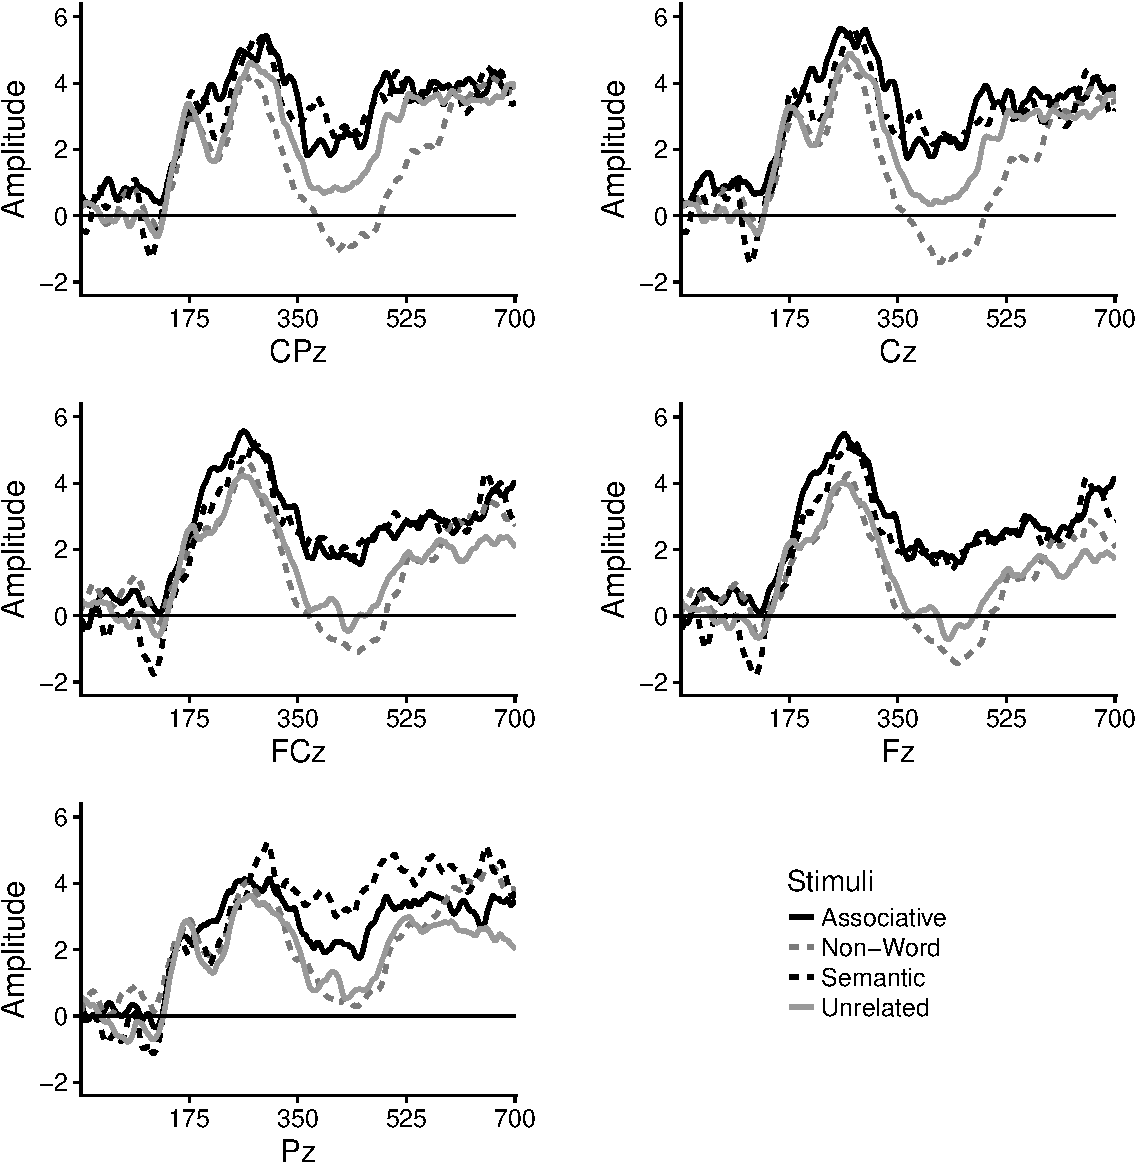
\includegraphics{BrainPaper_files/figure-latex/graph-LDT-1.pdf}
\caption{\label{fig:graph-LDT}SOMETHING SOMETHING HERE}
\end{figure}

\begin{figure}
\centering
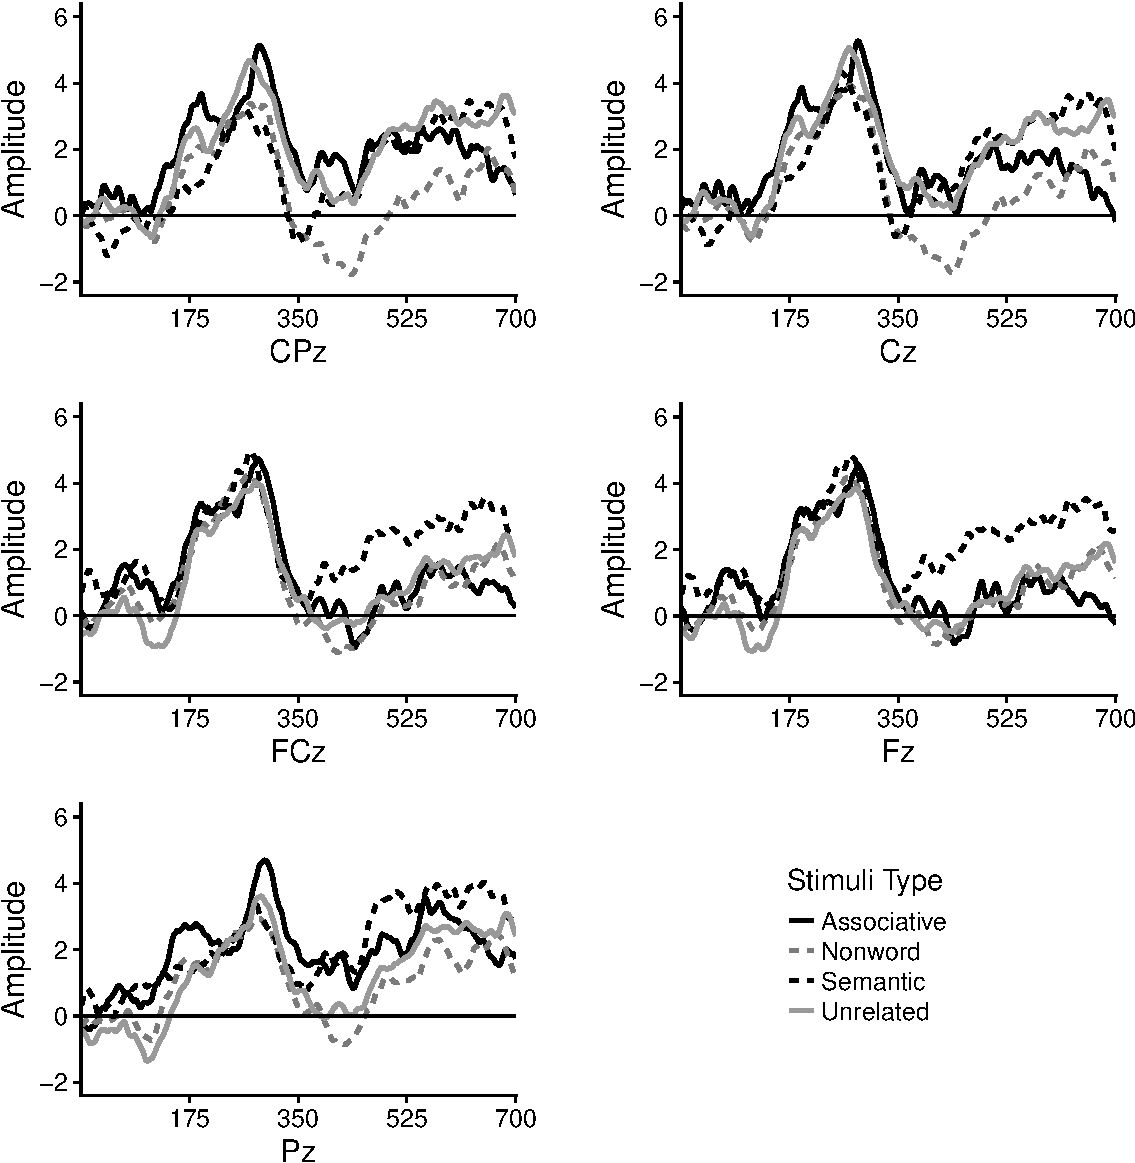
\includegraphics{BrainPaper_files/figure-latex/graph-LST-1.pdf}
\caption{\label{fig:graph-LST}SOMETHING SOMETHING HERE}
\end{figure}

\begin{table}[tbp]
\begin{center}
\begin{threeparttable}
\caption{\label{tab:area-table-model}Area under curve model statistics}
\begin{tabular}{lcccccc}
\toprule
Model & $df$ & AIC & BIC & $\chi^2$ & $\Delta\chi^2$ & $p$\\
\midrule
LDT Intercept & 2 & 5854.50 & 5862.27 & -2925.25 & NA & NA\\
LDT Random Intercept & 3 & 5639.91 & 5651.57 & -2816.96 & 216.59 & < .001\\
LDT Full & 10 & 5585.86 & 5624.72 & -2782.93 & 68.05 & < .001\\
LST Intercept & 2 & 5704.00 & 5711.75 & -2850.00 & NA & NA\\
LST Random Intercept & 3 & 5443.21 & 5454.85 & -2718.61 & 262.78 & < .001\\
LST Full & 10 & 5435.82 & 5474.60 & -2707.91 & 21.39 & .003\\
\bottomrule
\addlinespace
\end{tabular}
\begin{tablenotes}[para]
\textit{Note.} AIC: Aikaike Information Criterion, BIC: Bayesian Information Criterion
\end{tablenotes}
\end{threeparttable}
\end{center}
\end{table}

\begin{table}[tbp]
\begin{center}
\begin{threeparttable}
\caption{\label{tab:area-table-est}Area under curve model estimates}
\begin{tabular}{lccccc}
\toprule
Task & Predictor & $b$ & $SE$ & $t$ & $p$\\
\midrule
LDT & CZ & -59.86 & 85.35 & -0.70 & .484\\
LDT & FCZ & -124.76 & 85.35 & -1.46 & .145\\
LDT & FZ & -173.07 & 85.35 & -2.03 & .043\\
LDT & PZ & 54.22 & 85.35 & 0.64 & .526\\
LDT & Unrelated - Nonword & -189.97 & 76.34 & -2.49 & .013\\
LDT & Unrelated - Semantic & 331.30 & 76.34 & 4.34 & < .001\\
LDT & Unrelated - Associative & 301.18 & 76.34 & 3.95 & < .001\\
LDT & Nonword - Semantic & 521.27 & 76.34 & 6.83 & < .001\\
LDT & Nonword - Associative & 491.15 & 76.34 & 6.43 & < .001\\
LDT & Semantic - Associative & -30.12 & 76.34 & -0.39 & .693\\
LST & CZ & -38.69 & 73.85 & -0.52 & .601\\
LST & FCZ & -61.36 & 73.58 & -0.83 & .405\\
LST & FZ & -50.44 & 73.58 & -0.69 & .493\\
LST & PZ & 12.85 & 74.14 & 0.17 & .862\\
LST & Unrelated - Nonword & -184.82 & 65.81 & -2.81 & .005\\
LST & Unrelated - Semantic & 91.03 & 66.01 & 1.38 & .169\\
LST & Unrelated - Associative & 43.60 & 66.21 & 0.66 & .511\\
LST & Nonword - Semantic & 275.86 & 66.01 & 4.18 & < .001\\
LST & Nonword - Associative & 228.43 & 66.21 & 3.45 & .001\\
LST & Semantic - Associative & -47.43 & 66.41 & -0.71 & .476\\
\bottomrule
\addlinespace
\end{tabular}
\begin{tablenotes}[para]
\textit{Note.} The site control level was considered CPZ. Degrees of freedom are 335 for lexical decision tasks and 332 for letter search tasks.
\end{tablenotes}
\end{threeparttable}
\end{center}
\end{table}

\subsection{Task Performance}\label{task-performance}

One persons data was corrupt for the complete task component, and one
participant's task excluded several of their responses. The missing
responses were excluded for this analysis (\emph{n} = 16 complete with
360 responses, \emph{n} = 1 with 329 responses). Task data were scored
for correctness in the two tasks, and overall performance was around
94\% for each task: LDT, \emph{M} = 94.38 (\emph{SD} = 23.03) and LST,
\emph{M} = 94.38 (\emph{SD} = 23.03). Incorrect trials (\emph{n} = 335)
were discarded for the response latency analysis. An analysis of
outliers indicated there were 214 trials with long response latencies,
and they were excluded from the analysis.

Two MLM analyses were conducted on each task separately, with stimuli as
the independent variable and response latency as the dependent variable,
controlling for participants as a random factor (see Table
\ref{tab:RT-table-model}). In both the lexical decision and letter
search tasks, there were significant improvements in the model by
including stimuli as a predictor over the random intercept model,
\emph{p}s \textless{} .001. Each stimuli type was compared pairwise, and
\(\alpha\) was again set at .008 to control the Type I error rate. Table
\ref{tab:RT-table-est} includes these comparisons from the dummy coded
models, and means with 95\% confidence intervals are displayed in Figure
\ref{fig:RT-graph}. For the lexical decision task, nonwords were slower
than all other stimuli types. Unrelated words were not different from
semantic word pairs, but were slower than associative word pairs. This
finding indicated that the lexical decision task showed associative
priming, but not semantic priming; however, there were not response
latency differences for these two related word pair types. In contrast
to this finding, and results from the N400 area under the curves, we
found priming for both semantic and associative word pairs in the letter
search task. Nonwords were again slower than all other stimuli types,
followed by unrelated word pairs. Again, semantic and associative pairs
were not different. These analyses were examined with the outliers
included in the analysis, as we considered that eliminating 214 trials
may have skewed the results. The pattern of results did not change, but
the differences between unrelated pairs and other stimuli types do
become larger.

\begin{table}[tbp]
\begin{center}
\begin{threeparttable}
\caption{\label{tab:RT-table-model}Response latency model statistics}
\begin{tabular}{lcccccc}
\toprule
Model & $df$ & AIC & BIC & $\chi^2$ & $\Delta\chi^2$ & $p$\\
\midrule
LDT Intercept & 2 & 43019.73 & 43031.59 & -21507.87 & NA & NA\\
LDT Random Intercept & 3 & 42613.48 & 42631.25 & -21303.74 & 408.26 & < .001\\
LDT Full & 6 & 42443.72 & 42479.27 & -21215.86 & 175.76 & < .001\\
LST Intercept & 2 & 45000.97 & 45012.82 & -22498.48 & NA & NA\\
LST Random Intercept & 3 & 44365.19 & 44382.97 & -22179.60 & 637.78 & < .001\\
LST Full & 6 & 44286.21 & 44321.77 & -22137.10 & 84.98 & < .001\\
\bottomrule
\addlinespace
\end{tabular}
\begin{tablenotes}[para]
\textit{Note.} AIC: Aikaike Information Criterion, BIC: Bayesian Information Criterion
\end{tablenotes}
\end{threeparttable}
\end{center}
\end{table}

\begin{table}[tbp]
\begin{center}
\begin{threeparttable}
\caption{\label{tab:RT-table-est}Response latency model estimates}
\begin{tabular}{lccccc}
\toprule
Task & Predictor & $b$ & $SE$ & $t$ & $p$\\
\midrule
LDT & Unrelated - Nonword & 246.80 & 24.20 & 10.20 & < .001\\
LDT & Unrelated - Semantic & -13.89 & 28.78 & -0.48 & .629\\
LDT & Unrelated - Associative & -96.63 & 28.62 & -3.38 & .001\\
LDT & Nonword - Semantic & -260.69 & 29.32 & -8.89 & < .001\\
LDT & Nonword - Associative & -343.43 & 29.15 & -11.78 & < .001\\
LDT & Semantic - Associative & -82.74 & 33.06 & -2.50 & .012\\
LST & Unrelated - Nonword & 134.48 & 32.95 & 4.08 & < .001\\
LST & Unrelated - Semantic & -201.81 & 39.48 & -5.11 & < .001\\
LST & Unrelated - Associative & -122.49 & 39.48 & -3.10 & .002\\
LST & Nonword - Semantic & -336.29 & 39.71 & -8.47 & < .001\\
LST & Nonword - Associative & -256.98 & 39.71 & -6.47 & < .001\\
LST & Semantic - Associative & 79.31 & 45.28 & 1.75 & .080\\
\bottomrule
\addlinespace
\end{tabular}
\begin{tablenotes}[para]
\textit{Note.} Degrees of freedom are 2747 for lexical decision tasks and 2753 for letter search tasks.
\end{tablenotes}
\end{threeparttable}
\end{center}
\end{table}

\begin{figure}
\centering
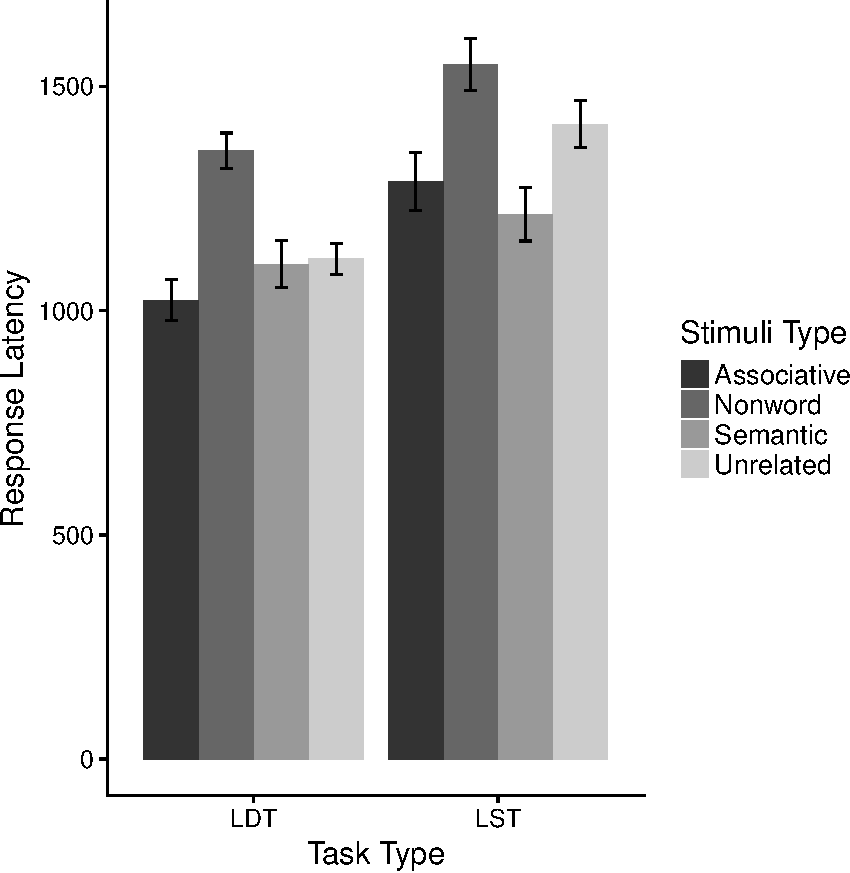
\includegraphics{BrainPaper_files/figure-latex/RT-graph-1.pdf}
\caption{\label{fig:RT-graph}SOMETHING SOMETHING HERE}
\end{figure}

\section{Discussion}\label{discussion}

These experiments were designed to explore the differences between N400
activation in the brain following presentation of semantic-only,
associative-only, and unrelated word pairs in priming tasks. The N400
data and reaction time data present picture of associative and semantic
priming during both lexical decision and letter search task. Because
both tasks were designed to reduce controlled processing of cue-target
relationships, these findings imply automatic activation of word
meanings and associations, even when task demands do not warrant word
activation. Nonword activation is more problematic to interpret, as N400
waveforms are not different from unrelated word pairs, but reaction time
data is much slower. These results, taken together, may illustrate a
controlled process search of the lexicon requiring the same activation
levels. When an unrelated target word is found in the lexicon,
controlled search is terminated, while searching for a nonword continues
for more time before the search is terminated. However, Deacon et al.
(2000) point to potential issues with the relationship between the N400
and automaticity. Semantic processing, Deacon et al. (2000) discuss, is
possible in the absence of attention or a dearth of awareness.

Since findings were roughly similar for associative and semantic word
pairs, we can postulate that the activation processes for these types of
word relatedness are also roughly similar. This experiment cannot
separate if the cognitive architecture is different for associations and
semantics, but that the automatic mechanisms for priming are comparable.
One limitation is that the long stimulus onset times may have allowed
for controlled processing in the reaction time data, but the consistent
N400 attenuation suggests a quick search of the lexicon similar to an
automatic activation process. Finally, differences in activation across
gender need to be explored. Although not conclusive due to sample size,
we found that male activation across stimuli was implicated in
traditional left Broca?s area, while female activation averaged to
central parietal areas. Regardless of any potential differences, the
broad sensitivity of the N400 means it can be implemented when
investigating how information is stored in the brain. The temporal lobe
has been shown to be implicated as a source from the N400, albeit occurs
in a flexible manner, varying with different classes of stimuli
(Federmeier \& Laszlo, 2009). There are sometimes dissociations between
the N400 and reaction time measures. The use of the N400 can therefore
be seen as an especially relevant dependent measure for the reason that
components can only partially be a reflection of semantic processes
relating to response latencies (Kutas \& Federmeier, 2011).

To date, research has focused on semantic priming and its automaticity
without many controls for associative relationships embedded in word
pairs. Certainly there is overlap between meaning and context use of
words, but these differences can be studied separately using available
databases (Hutchison, 2003). Our current study has supported findings by
Marí-Beffa et al. (2005), who showed activation during letter search
tasks, along with the many studies on automatic activation during masked
priming (Deacon et al., 2000; Kiefer, 2002).

Limitations do exist within these experiments. As previously mentioned a
larger sample size would increase the power coefficient of the findings.
Future studies should focus on the extent of priming in semantic word
pairs during a letter search task, which is a controversial topic within
the literature. Since our study limited relatedness to associations or
semantics, upcoming experiments could examine the interaction between
word relationship type of N400 attenuation. Kreher, Holcomb, and
Kuperberg (2006) have shown that N400 waveform differences can be
attributed to different strengths of semantic relatedness in a linear
fashion. With more exploration into the exact priming nature of
associations and semantics, we may begin to discover their cognitive
mechanisms.

\newpage

\section{References}\label{references}

\setlength{\parindent}{-0.5in} \setlength{\leftskip}{0.5in}

\hypertarget{refs}{}
\hypertarget{ref-Brown1993}{}
Brown, C., \& Hagoort, P. (1993). The processing nature of the N400:
Evidence from masked priming. \emph{Journal of Cognitive Neuroscience},
\emph{5}(1), 34--44.
doi:\href{https://doi.org/10.1162/jocn.1993.5.1.34}{10.1162/jocn.1993.5.1.34}

\hypertarget{ref-Buchanan2010}{}
Buchanan, E. M. (2010). Access into Memory: Differences in Judgments and
Priming for Semantic and Associative Memory. \emph{Journal of Scientific
Psychology}, (March), 1--8.

\hypertarget{ref-Buchanan2013}{}
Buchanan, E. M., Holmes, J. L., Teasley, M. L., \& Hutchison, K. A.
(2013). English semantic word-pair norms and a searchable Web portal for
experimental stimulus creation. \emph{Behavior Research Methods},
\emph{45}(3), 746--757.
doi:\href{https://doi.org/10.3758/s13428-012-0284-z}{10.3758/s13428-012-0284-z}

\hypertarget{ref-Collins1975}{}
Collins, A. M., \& Loftus, E. F. (1975). A spreading-activation theory
of semantic processing. \emph{Psychological Review}, \emph{82}(6),
407--428.
doi:\href{https://doi.org/10.1037//0033-295X.82.6.407}{10.1037//0033-295X.82.6.407}

\hypertarget{ref-Deacon2004}{}
Deacon, D., Dynowska, A., Ritter, W., \& Grose-Fifer, J. (2004).
Repetition and semantic priming of nonwords: Implications for theories
of N400 and word recognition. \emph{Psychophysiology}, \emph{41}(1),
60--74.
doi:\href{https://doi.org/10.1111/1469-8986.00120}{10.1111/1469-8986.00120}

\hypertarget{ref-Deacon2000}{}
Deacon, D., Hewitt, S., Yang, C.-M., \& Nagata, M. (2000). Event-related
potential indices of semantic priming using masked and unmasked words:
evidence that the N400 does not reflect a post-lexical process.
\emph{Cognitive Brain Research}, \emph{9}(2), 137--146.
doi:\href{https://doi.org/10.1016/S0926-6410(99)00050-6}{10.1016/S0926-6410(99)00050-6}

\hypertarget{ref-Federmeier2009}{}
Federmeier, K. D., \& Laszlo, S. (2009). Time for meaning:
Electrophysiology provides insights into dynamics of representation and
processing in semantic memory. In B. H. Ross (Ed.), \emph{Psychology of
learning and motivation} (pp. 1--44). Burlington, MA: Academic Press.

\hypertarget{ref-Felbaum1998}{}
Felbaum, C. (1998). \emph{WordNet: An Electronic Lexical Database}. MIT
Press.

\hypertarget{ref-Ford1983}{}
Ford, M. (1983). A method for obtaining measures of local parsing
complexity throughout sentences. \emph{Journal of Verbal Learning and
Verbal Behavior}, \emph{22}(2), 203--218.
doi:\href{https://doi.org/10.1016/S0022-5371(83)90156-1}{10.1016/S0022-5371(83)90156-1}

\hypertarget{ref-Friedrich1991}{}
Friedrich, F. J., Henik, A., \& Tzelgov, J. (1991). Automatic processes
in lexical access and spreading activation. \emph{Journal of
Experimental Psychology: Human Perception and Performance},
\emph{17}(3), 792--806.
doi:\href{https://doi.org/10.1037//0096-1523.17.3.792}{10.1037//0096-1523.17.3.792}

\hypertarget{ref-Gelman2006}{}
Gelman, A. (2006). Multilevel (hierarchical) modeling: What it can and
cannot do. \emph{Technometrics}, \emph{48}(3), 432--435.
doi:\href{https://doi.org/10.1198/004017005000000661}{10.1198/004017005000000661}

\hypertarget{ref-Hagoort2009}{}
Hagoort, P., Baggio, G., \& Willems, R. M. (2009). Semantic unification.
In M. S. Gazzaniga (Ed.), \emph{The cognitive neurosciences} (4th ed.,
pp. 819--836). Cambridge, MA: MIT Press.

\hypertarget{ref-Hutchison2003}{}
Hutchison, K. A. (2003). Is semantic priming due to association strength
or feature overlap? A microanalytic review. \emph{Psychonomic Bulletin
\& Review}, \emph{10}(4), 785--813.
doi:\href{https://doi.org/10.3758/BF03196544}{10.3758/BF03196544}

\hypertarget{ref-Jiang1997}{}
Jiang, J. J., \& Conrath, D. W. (1997). Semantic similarity based on
corpus statistics and lexical taxonomy. In \emph{In proceedings of
international conference research on computational linguistics (rocling
x)}. Taiwan.

\hypertarget{ref-Kiefer2002}{}
Kiefer, M. (2002). The N400 is modulated by unconsciously perceived
masked words: further evidence for an automatic spreading activation
account of N400 priming effects. \emph{Cognitive Brain Research},
\emph{13}(1), 27--39.
doi:\href{https://doi.org/10.1016/S0926-6410(01)00085-4}{10.1016/S0926-6410(01)00085-4}

\hypertarget{ref-Kreher2006}{}
Kreher, D. A., Holcomb, P. J., \& Kuperberg, G. R. (2006). An
electrophysiological investigation of indirect semantic priming.
\emph{Psychophysiology}, \emph{43}(6), 550--563.
doi:\href{https://doi.org/10.1111/j.1469-8986.2006.00460.x}{10.1111/j.1469-8986.2006.00460.x}

\hypertarget{ref-Kutas2000}{}
Kutas, M., \& Federmeier, K. D. (2000). Electrophysiology reveals
semantic memory use in language comprehension. \emph{Trends in Cognitive
Sciences}, \emph{4}(12), 463--470.
doi:\href{https://doi.org/10.1016/S1364-6613(00)01560-6}{10.1016/S1364-6613(00)01560-6}

\hypertarget{ref-Kutas2011}{}
Kutas, M., \& Federmeier, K. D. (2011). Thirty years and counting:
Finding meaning in the N400 component of the Event-Related Brain
Potential (ERP). \emph{Annual Review of Psychology}, \emph{62}(1),
621--647.
doi:\href{https://doi.org/10.1146/annurev.psych.093008.131123}{10.1146/annurev.psych.093008.131123}

\hypertarget{ref-Lucas2000}{}
Lucas, M. (2000). Semantic priming without association: A meta-analytic
review. \emph{Psychonomic Bulletin \& Review}, \emph{7}(4), 618--630.
doi:\href{https://doi.org/10.3758/BF03212999}{10.3758/BF03212999}

\hypertarget{ref-Maki2008}{}
Maki, W. S., \& Buchanan, E. M. (2008). Latent structure in measures of
associative, semantic, and thematic knowledge. \emph{Psychonomic
Bulletin \& Review}, \emph{15}(3), 598--603.
doi:\href{https://doi.org/10.3758/PBR.15.3.598}{10.3758/PBR.15.3.598}

\hypertarget{ref-Maki2004}{}
Maki, W. S., McKinley, L. N., \& Thompson, A. G. (2004). Semantic
distance norms computed from an electronic dictionary (WordNet).
\emph{Behavior Research Methods, Instruments, \& Computers},
\emph{36}(3), 421--431.
doi:\href{https://doi.org/10.3758/BF03195590}{10.3758/BF03195590}

\hypertarget{ref-Mari-Beffa2005}{}
Marí-Beffa, P., Valdés, B., Cullen, D. J., Catena, A., \& Houghton, G.
(2005). ERP analyses of task effects on semantic processing from words.
\emph{Cognitive Brain Research}, \emph{23}(2-3), 293--305.
doi:\href{https://doi.org/10.1016/j.cogbrainres.2004.10.016}{10.1016/j.cogbrainres.2004.10.016}

\hypertarget{ref-McRae2005}{}
McRae, K., Cree, G. S., Seidenberg, M. S., \& McNorgan, C. (2005).
Semantic feature production norms for a large set of living and
nonliving things. \emph{Behavior Research Methods}, \emph{37}(4),
547--559.
doi:\href{https://doi.org/10.3758/BF03192726}{10.3758/BF03192726}

\hypertarget{ref-Meyer1971}{}
Meyer, D. E., \& Schvaneveldt, R. W. (1971). Facilitation in recognizing
pairs of words: Evidence of a dependence between retrieval operations.
\emph{Journal of Experimental Psychology}, \emph{90}(2), 227--234.
doi:\href{https://doi.org/10.1037/h0031564}{10.1037/h0031564}

\hypertarget{ref-Miller1991}{}
Miller, J. (1991). Short report: Reaction time analysis with outlier
exclusion: Bias varies with sample size. \emph{The Quarterly Journal of
Experimental Psychology Section A}, \emph{43}(4), 907--912.
doi:\href{https://doi.org/10.1080/14640749108400962}{10.1080/14640749108400962}

\hypertarget{ref-Moss1995}{}
Moss, H. E., Ostrin, R. K., Tyler, L. K., \& Marslen-Wilson, W. D.
(1995). Accessing different types of lexical semantic information:
Evidence from priming. \emph{Journal of Experimental Psychology:
Learning, Memory, and Cognition}, \emph{21}(4), 863--883.
doi:\href{https://doi.org/10.1037//0278-7393.21.4.863}{10.1037//0278-7393.21.4.863}

\hypertarget{ref-Neely1991}{}
Neely, J. H. (1991). \emph{Semantic priming effects in visual word
recognition: A selective review of current findings and theories}.
Hillsdale, NJ: Lawrence Erlbaum Associates, Inc.

\hypertarget{ref-Nelson2004}{}
Nelson, D. L., McEvoy, C. L., \& Schreiber, T. A. (2004). The University
of South Florida free association, rhyme, and word fragment norms.
\emph{Behavior Research Methods, Instruments, \& Computers},
\emph{36}(3), 402--407.
doi:\href{https://doi.org/10.3758/BF03195588}{10.3758/BF03195588}

\hypertarget{ref-Patwardhan2003}{}
Patwardhan, S., Banerjee, S., \& Pedersen, T. (2003). Using measures of
semantic relatedness for word sense disambiguation. In \emph{Proceedings
of the fourth international conference on intelligent text processing
and computational linguistics} (Vol. 4, pp. 241--257). Springer, Berlin,
Heidelberg.
doi:\href{https://doi.org/10.1007/3-540-36456-0_24}{10.1007/3-540-36456-0\_24}

\hypertarget{ref-Pinheiro2017}{}
Pinheiro, J., Bates, D., Debroy, S., Sarkar, D., \& Team, R. C. (2017).
nlme: Linear and nonlinear mixed effects models. Retrieved from
\url{https://cran.r-project.org/package=nlme}

\hypertarget{ref-Rolke2001}{}
Rolke, B., Heil, M., Streb, J., \& Hennighausen, E. (2001). Missed prime
words within the attentional blink evoke an N400 semantic priming
effect. \emph{Psychophysiology}, \emph{38}(2), 165--174.
doi:\href{https://doi.org/10.1111/1469-8986.3820165}{10.1111/1469-8986.3820165}

\hypertarget{ref-Smith2001}{}
Smith, M. C., \& Besner, D. (2001). Modulating semantic feedback in
visual word recognition. \emph{Psychonomic Bulletin \& Review},
\emph{8}(1), 111--117.
doi:\href{https://doi.org/10.3758/BF03196146}{10.3758/BF03196146}

\hypertarget{ref-Stolz1996a}{}
Stolz, J. A., \& Besner, D. (1996). Role of set in visual word
recognition: Activation and activation blocking as nonautomatic
processes. \emph{Journal of Experimental Psychology: Human Perception
and Performance}, \emph{22}(5), 1166--1177.
doi:\href{https://doi.org/10.1037//0096-1523.22.5.1166}{10.1037//0096-1523.22.5.1166}

\hypertarget{ref-Tse2007}{}
Tse, C.-S., \& Neely, J. H. (2007). Semantic priming from
letter-searched primes occurs for low- but not high-frequency targets:
Automatic semantic access may not be a myth. \emph{Journal of
Experimental Psychology: Learning, Memory, and Cognition}, \emph{33}(6),
1143--1161.
doi:\href{https://doi.org/10.1037/0278-7393.33.6.1143}{10.1037/0278-7393.33.6.1143}

\hypertarget{ref-VanSelst1994}{}
Van Selst, M., \& Jolicoeur, P. (1994). Can mental rotation occur before
the dual-task bottleneck? \emph{Journal of Experimental Psychology:
Human Perception and Performance}, \emph{20}(4), 905--921.
doi:\href{https://doi.org/10.1037/0096-1523.20.4.905}{10.1037/0096-1523.20.4.905}

\hypertarget{ref-Vinson2008}{}
Vinson, D. P., \& Vigliocco, G. (2008). Semantic feature production
norms for a large set of objects and events. \emph{Behavior Research
Methods}, \emph{40}(1), 183--190.
doi:\href{https://doi.org/10.3758/BRM.40.1.183}{10.3758/BRM.40.1.183}






\end{document}
